% CS 111 style
% Typical usage (all UPPERCASE items are optional):
%       \input 111pre
%       \begin{document}
%       \MYTITLE{Title of document, e.g., Lab 1\\Due ...}
%       \MYHEADERS{short title}{other running head, e.g., due date}
%       \PURPOSE{Description of purpose}
%       \SUMMARY{Very short overview of assignment}
%       \DETAILS{Detailed description}
%         \SUBHEAD{if needed} ...
%         \SUBHEAD{if needed} ...
%          ...
%       \HANDIN{What to hand in and how}
%       \begin{checklist}
%       \item ...
%       \end{checklist}
% There is no need to include a "\documentstyle."
% However, there should be an "\end{document}."
%
%===========================================================
\documentclass[11pt,twoside,titlepage]{article}
%%NEED TO ADD epsf!!
\usepackage{threeparttop}
\usepackage{graphicx}
\usepackage{latexsym}
\usepackage{color}
\usepackage{listings}
\usepackage{fancyvrb}
%\usepackage{pgf,pgfarrows,pgfnodes,pgfautomata,pgfheaps,pgfshade}
\usepackage{tikz}
\usepackage[normalem]{ulem}
\tikzset{
    %Define standard arrow tip
%    >=stealth',
    %Define style for boxes
    oval/.style={
           rectangle,
           rounded corners,
           draw=black, very thick,
           text width=6.5em,
           minimum height=2em,
           text centered},
    % Define arrow style
    arr/.style={
           ->,
           thick,
           shorten <=2pt,
           shorten >=2pt,}
}
\usepackage[noend]{algorithmic}
\usepackage[noend]{algorithm}
\newcommand{\bfor}{{\bf for\ }}
\newcommand{\bthen}{{\bf then\ }}
\newcommand{\bwhile}{{\bf while\ }}
\newcommand{\btrue}{{\bf true\ }}
\newcommand{\bfalse}{{\bf false\ }}
\newcommand{\bto}{{\bf to\ }}
\newcommand{\bdo}{{\bf do\ }}
\newcommand{\bif}{{\bf if\ }}
\newcommand{\belse}{{\bf else\ }}
\newcommand{\band}{{\bf and\ }}
\newcommand{\breturn}{{\bf return\ }}
\newcommand{\mod}{{\rm mod}}
\renewcommand{\algorithmiccomment}[1]{$\rhd$ #1}
\newenvironment{checklist}{\par\noindent\hspace{-.25in}{\bf Checklist:}\renewcommand{\labelitemi}{$\Box$}%
\begin{itemize}}{\end{itemize}}
\pagestyle{threepartheadings}
\usepackage{url}
\usepackage{wrapfig}
% \usepackage{hyperref}
\usepackage[hidelinks]{hyperref}
%=========================
% One-inch margins everywhere
%=========================
\setlength{\topmargin}{0in}
\setlength{\textheight}{8.5in}
\setlength{\oddsidemargin}{0in}
\setlength{\evensidemargin}{0in}
\setlength{\textwidth}{6.5in}
%===============================
%===============================
% Macro for document title:
%===============================
\newcommand{\MYTITLE}[1]%
   {\begin{center}
     \begin{center}
     \bf
     CMPSC 111\\Introduction to Computer Science I\\
     Fall 2014\\
     \medskip
     \end{center}
     \bf
     #1
     \end{center}
}
%================================
% Macro for headings:
%================================
\newcommand{\MYHEADERS}[2]%
   {\lhead{#1}
    \rhead{#2}
    \immediate\write16{}
    \immediate\write16{DATE OF HANDOUT?}
    \read16 to \dateofhandout
    \lfoot{\sc Handed out on \dateofhandout}
    \immediate\write16{}
    \immediate\write16{HANDOUT NUMBER?}
    \read16 to\handoutnum
    \rfoot{Handout \handoutnum}
   }

%================================
% Macro for bold italic:
%================================
\newcommand{\bit}[1]{{\textit{\textbf{#1}}}}

%=========================
% Non-zero paragraph skips.
%=========================
\setlength{\parskip}{1ex}

%=========================
% Create various environments:
%=========================
\newcommand{\PURPOSE}{\par\noindent\hspace{-.25in}{\bf Purpose:\ }}
\newcommand{\SUMMARY}{\par\noindent\hspace{-.25in}{\bf Summary:\ }}
\newcommand{\DETAILS}{\par\noindent\hspace{-.25in}{\bf Details:\ }}
\newcommand{\HANDIN}{\par\noindent\hspace{-.25in}{\bf Hand in:\ }}
\newcommand{\SUBHEAD}[1]{\bigskip\par\noindent\hspace{-.1in}{\sc #1}\\}
%\newenvironment{CHECKLIST}{\begin{itemize}}{\end{itemize}}

\begin{document}
\MYTITLE{Lab 8 for Sections 03 and 04 \\ 30 October 2014\\
Due Thursday, 6 November by 2:30pm }

\vspace{-0.2in}
\subsection*{Objectives}
\vspace{-0.05in}

To enhance your experience with designing and implementing your own Java classes, including the completion of tasks such
as picking the right instance variables and creating both the constructors and the methods.  Additionally, to practice
using compound {\tt if/else} statements as part of a solution to a real-world problem involving a popular and well-known
game.

\vspace{-0.15in}
\subsection*{General Guidelines for Labs}
\vspace{-0.05in}
\begin{itemize}
\item
{\bf Work on the Alden Hall computers.} If you want to work on a different
machine, be sure to transfer your programs to the Alden
machines and re-run them before submitting.
\item
  {\bf Update your repository often!} You should {\tt add}, {\tt commit}, 
  and {\tt push} your updated files each time you work on them.  I will not grade 
your programs until the due date has passed.
\item
{\bf Review the Honor Code policy.} You
may discuss programs with others, but programs that are nearly identical
to others will be taken as evidence of violating the Honor Code.
\end{itemize}

\vspace{-0.15in}
\subsection*{Reading Assignment}
\vspace{-0.05in}

To learn more about {\tt if} statement and boolean expressions, review Sections 5.1--5.3; to recall material on
constructing classes and methods, read Sections 4.1--4.5.  Students who are not familiar with the Sudoku game are
encouraged to examine \url{http://en.wikipedia.org/wiki/Sudoku}.

\vspace{-0.1in}
\subsection*{Create a New Directory and Two Java Programs}
\vspace{-0.05in}

In your own {\tt cs111F2014-<your user name>} repository inside the {\tt labs/} directory, create a directory called
{\tt lab8}. Type ``{\tt cd lab8}'' to move to the new directory. Then, using {\tt gvim}, you should create {\tt
  SudokuChecker.java} and {\tt SudokuCheckerMain.java} files that will store your solution to this laboratory
assignment. Remember to use the Java program template from a previous lab!

\vspace{-0.1in}
\subsection*{Implementing a Sudoku Checker}
\vspace{-0.05in}

Sudoku is a logic-based placement puzzle. The aim of this puzzle is to enter a numerical digit from 1 through 9 in each
cell of a 9x9 grid made up of 3x3 subgrids (called the ``regions''), starting with various digits given in some cells
(called the ``givens''). Each row, column, and region must contain only one instance of each valid numeral.

\noindent For this lab, you are going to write a Sudoku validator for 4x4 grids made up of 2x2 regions instead of 9x9
grids made up of 3x3 regions.  In contrast to the previously explained full grids, Sudoku puzzles that use 4x4 grids
only use the numerical digits 1 through 4 instead of 1 through 9.

\noindent Here are two correct 4x4 Sudoku grids:

\vspace*{.01in}
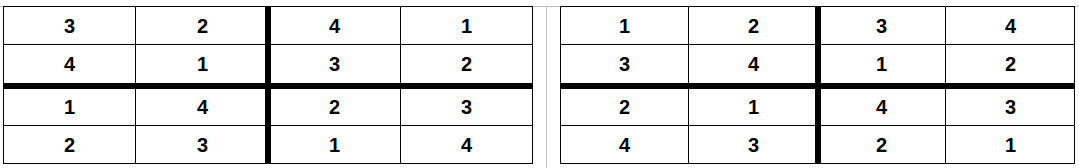
\includegraphics[scale=0.3]{grids}

\noindent Notice how each row, column, and region has the individual numbers from 1 through 4 used only once.  This means
that the values used in each row, column, and region must add up to 10 because of the fact that (1 + 2 + 3 + 4) = 10.  This is
how your program will check the 4x4 Sudoku grids.

\noindent Your program should allow its user to enter their Sudoku grids row-by-row, requiring that they separate each
of the four values by a space and that they hit ENTER at the end of the row.

\noindent When the user has entered all 16 values into the program, you should output validation checks for each region,
row, and column.  An example run of ``{\tt SudokuChecker}'' can be seen below.

\begin{verbatim}
Welcome to the Sudoku Checker!

This program checks simple and small 4x4 Sudoku grids for correctness. 
Each column, row, and 2x2 region contains the numbers 1 through 4 only once.

To check your Sudoku, enter your board one row at a time, 
with each digit separated by a space.  Hit ENTER at the end of a row.

Enter Row 1: 3 2 4 1
Enter Row 2: 4 1 3 2
Enter Row 3: 1 4 2 3
Enter Row 4: 2 3 1 4

REG-1:GOOD
REG-2:GOOD
REG-3:GOOD
REG-4:GOOD

ROW-1:GOOD
ROW-2:GOOD
ROW-3:GOOD
ROW-4:GOOD

COL-1:GOOD
COL-2:GOOD
COL-3:GOOD
COL-4:GOOD

SUDOKU GRID IS VALID!
\end{verbatim}

\newpage

\noindent Your program does not have to check for the numbers 1 through 4 being used uniquely in each row, column, and
region.  In other words, don't worry about validating the user's input to make sure they only enter the digits 1, 2, 3,
or 4 and only enter them once per row, column, and region.  You simply need to check that each row, column, and region
adds up to 10. This simplistic type of checking will, however, allow some bad Sudoku grids to be validated as
good---this is acceptable. 

\noindent Rows, columns, and regions are identified as found below:\\

\vspace*{.01in}
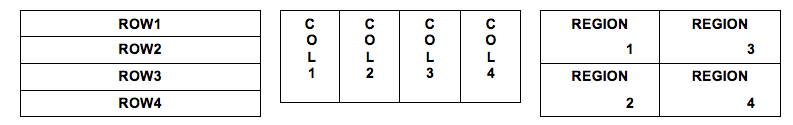
\includegraphics[scale=0.5]{sud}

\subsubsection*{{\tt SudokuCheckerMain} Class}

To use the {\tt SudokuChecker} class, follow this template for the {\tt SudokuCheckerMain.java} file:
\begin{verbatim}
public class SudokuCheckerMain
{
     public static void main ( String args[] )
     {
          SudokuChecker checker = new SudokuChecker();
          // TODO: output the required welcome message
          checker.getGrid();
          checker.checkGrid();
     }
}
\end{verbatim}

\subsubsection*{{\tt SudokuChecker} Class}

\noindent The basic structure of {\tt SudokuChecker.java} is as follows:
\begin{verbatim}
import java.util.Scanner;

public class SudokuChecker
{
     // TODO: put private data members here
     // TODO: put constructor here
     // TODO: put getGrid() here
     // TODO: put checkGrid() here
}
\end{verbatim}
The UML diagram for {\tt SudokuChecker} is:
\begin{tabular}{|l|}
\hline
\textbf{SudokuChecker} \\
\hline
- w1 : Integer\\
- w2 : Integer\\
- w3 : Integer\\
- w4 : Integer\\
- x1 : Integer\\
- x2 : Integer\\
- x3 : Integer\\
- x4 : Integer\\
- y1 : Integer\\
- y2 : Integer\\
- y3 : Integer\\
- y4 : Integer\\
- z1 : Integer\\
- z2 : Integer\\
- z3 : Integer\\
- z4 : Integer\\
\hline
$<<constructor>>$ SudokuChecker( )\\
\hline
+ getGrid ( )\\
+ checkGrid ( )\\
\hline
\end{tabular}

\vspace*{.05in}
\noindent This is a short description of what each data member represents and what each method does:\\

\begin{tabular}{|l|p{10cm}|}
\hline
{\tt w1, w2, w3, w4} &  \\
{\tt x1, x2, x3, x4} & \\
{\tt y1, y2, y3, y4} & \\
{\tt z1, z2, z3, z4}	&  Private data members that will store the numbers the user inputs.  Variables {\tt w1} through {\tt w4}
are for the first row, {\tt x1} through {\tt x4} are for the second row
and so on. You should not have any other private data members in your class.\\
\hline
SudokuChecker()	&This is the constructor.  It should initialize each of the private data members to the value of 0, indicating
that the user has not yet assigned a value to the data member. \\
\hline

getGrid()	& This public method should read the Sudoku grid from the user row by row, using spaces between values in each row.\\
\hline 
checkGrid() &	This public method uses the private data members to test whether or not the given values are a valid Sudoku grid.\\
& Your method does not have to check for the numbers 1 through 4 being used uniquely in each row, column, and region.
In other words, don't worry about validating the user's input to make sure they only enter the digits 1, 2, 3, or 4 and only
enter them once per row, column, and region. \\ 
& When producing your output, you must first validate the regions, then the rows, and then the columns.  Each region,
row, and column validation should appear on a line by itself. \\
\hline
\end{tabular}

\vspace{-0.05in}
\subsection*{Points to Think About}
\vspace{-0.05in}

Since we have not talked about programming concepts such as arrays yet---in fact, you should not use them to complete
this assignment---you will need to input your 16 values into 16 separate variables.  Some suggestions would be {\tt w1},
{\tt w2}, {\tt w3}, and {\tt w4} for the first row and then {\tt x1}, {\tt x2}, {\tt x3}, and {\tt x4} for the second
row, and so on.  Once you validate that one row is good or not good, the rest of the program should essentially be a
matter of ``copy and paste'', replacing variables where appropriate.  The most challenging part of this program is
determining whether or not you have a good Sudoku configuration.  One suggestion would be to keep track of a
variable that counts the number of things that are invalid and, if that variable's value is 0 at the end of the program,
you have a valid Sudoku board. Please see the instructor if you have questions about these matters.

\vspace{-0.2in}
\subsection*{Additional Program Requirements}
\vspace{-0.05in}
\begin{itemize}
\item Make sure your program prints your name, the lab number, and the date. 
\item Make sure your program contains the comment header with the Honor Code pledge, your name, lab number, date, and the purpose of the program. 
\item Make sure your program is documented properly, with descriptive and useful comments throughout your program whenever appropriate. 
\item Make sure your output
  is neat (e.g., no missing spaces and no typos) and that your program is neatly formatted (e.g., the indenting is correct).
\item \textbf{You may not use array structures or loops for this assignment.}
\end{itemize}

\vspace{-0.2in}
\subsection*{Required Deliverables}
\vspace{-0.05in}

For this assignment you are invited to submit versions of the following deliverables through both the Bitbucket
repository and in a printed and signed format.

\vspace{-0.05in}
\begin{enumerate}
    \setlength{\itemsep}{0pt}
  \item Completed and properly formatted {\tt SudokuChecker.java} and {\tt SudokuCheckerMain.java} files.

  \item An output file containing outputs obtained from running {\tt SudokuCheckerMain} five times.
        
\end{enumerate}
\vspace{-0.05in}

\noindent As you complete this step, you should make sure that you created a {\tt lab8/} directory within your Git
repository.  Then, you can save all of the required deliverables in the {\tt lab8/} directory---please see the course
instructor or a teaching assistant if you are not able to create your directory properly. 

\noindent In addition to turning in signed and printed copies of your code and output, share your source code and the output
file with me through your Git repository by correctly using the ``{\tt git add}'', ``{\tt git commit}'', and ``{\tt git
  push}'' commands. When you are done, please ensure that the Bitbucket Web site has a {\tt lab8/} directory in your
repository with the two Java files in the list of deliverables and the {\tt output} file. Please see the instructor
if you have questions about assignment submission.

% In addition to turning in signed and printed copies of your code and output, please share your program and the output
% file with me through your Git repository by correctly using the ``{\tt git add}'', ``{\tt git commit}'', and ``{\tt git
% push}'' commands. When you are done, please ensure that the Bitbucket Web site has a {\tt lab8/} directory in your
% repository with the four files called {\tt Lab8.java}, {\tt Lab8Main.java}, and {\tt output}. You
% should see the instructor or a teaching assistant if you have questions about submitting this assignment.

In adherence to the Honor Code, students should complete this assignment on an individual basis. While it is appropriate
for students in this class to have high-level conversations about the assignment, it is necessary to distinguish
carefully between the student who discusses the principles underlying a problem with others and the student who produces
assignments that are identical to, or merely variations on, someone else's work.  Deliverables that are nearly identical
to the work of others will be taken as evidence of violating the \mbox{Honor Code}.  

\end{document}

\begin{verbatim}
Sample Run

Welcome to the Sudoku Checker v1.0!

This program checks simple, small, 4x4 Sudoku grids for correctness. Each column, row and 2x2 region contains the numbers 1 through 4 only once.

To check your Sudoku, enter your board one row at a time, with each digit separated by a space.  Hit ENTER at the end of a row.

Enter Row 1: 1 2 3 4
Enter Row 2: 3 4 2 1
Enter Row 3: 1 2 3 4
Enter Row 4: 4 3 2 1

Thank you.  Now checking ...

REG-1:GOOD
REG-2:GOOD
REG-3:GOOD
REG-4:GOOD
ROW-1:GOOD
ROW-2:GOOD
ROW-3:GOOD
ROW-4:GOOD
COL-1:BAD
COL-2:BAD
COL-3:GOOD
COL-4:GOOD

SUDO:INVALID



Sample Run
Welcome to the Sudoku Checker v1.0!

This program checks simple, small, 4x4 Sudoku grids for correctness. Each column, row and 2x2 region contains the numbers 1 through 4 only once.

To check your Sudoku, enter your board one row at a time, with each digit separated by a space.  Hit ENTER at the end of a row.

Enter Row 1: 3 2 4 1
Enter Row 2: 4 1 3 2
Enter Row 3: 1 4 2 3
Enter Row 4: 2 3 1 4

REG-1:GOOD
REG-2:GOOD
REG-3:GOOD
REG-4:GOOD
ROW-1:GOOD
ROW-2:GOOD
ROW-3:GOOD
ROW-4:GOOD
COL-1:GOOD
COL-2:GOOD
COL-3:GOOD
COL-4:GOOD

SUDO:VALID

\end{verbatim}



\end{document}
